\documentclass[aspectratio=169,10pt]{beamer}
\usetheme{Madrid}
\usepackage[T1]{fontenc}
\usepackage{lmodern}
\usepackage{tikz}
\usepackage{adjustbox}
\usetikzlibrary{arrows.meta,positioning,fit,backgrounds,calc,shadows}
\definecolor{prismNavy}{RGB}{13,29,54}
\definecolor{prismBlue}{RGB}{38,126,190}
\definecolor{prismTeal}{RGB}{28,161,157}
\definecolor{prismGold}{RGB}{229,166,50}
\setbeamercolor{frametitle}{bg=prismNavy,fg=white}
\setbeamertemplate{navigation symbols}{}
\setbeamertemplate{footline}{\hfill\insertshorttitle\hspace{1em}|\hspace{1em}\insertframenumber/\inserttotalframenumber\hspace{1em}\vspace{0.55em}}
\begin{document}
\begin{frame}[t]{PrismSpace architecture}
\vspace{-0.6em}
\centering
\maxsizebox{\linewidth}{0.78\textheight}{%
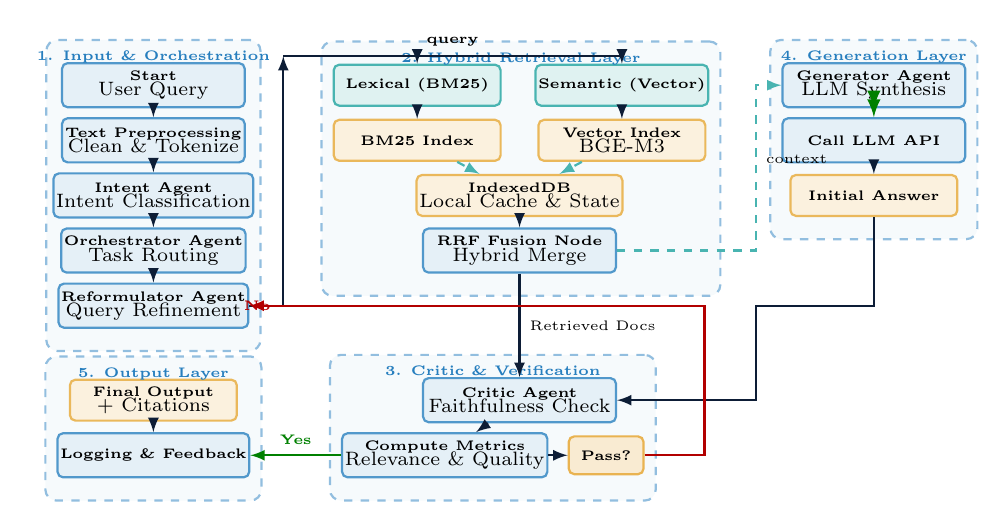
\begin{tikzpicture}[
  x=1cm, y=1cm,
  every node/.style={align=center, font=\tiny},
  layer/.style={draw=prismBlue!50, fill=prismBlue!4, rounded corners=4pt, thick, dashed, inner sep=4pt},
  maintitle/.style={font=\tiny\bfseries, text=prismBlue},
  mainbox/.style={draw=prismBlue!80, fill=prismBlue!12, rounded corners=2pt, thick,
    minimum width=2.32cm, minimum height=0.56cm, inner sep=1pt},
  subbox/.style={draw=prismTeal!80, fill=prismTeal!14, rounded corners=2pt, thick,
    minimum width=2.12cm, minimum height=0.52cm, inner sep=1pt},
  storage/.style={draw=prismGold!80, fill=prismGold!16, rounded corners=2pt, thick,
    minimum width=2.12cm, minimum height=0.52cm, inner sep=1pt},
  decide/.style={draw=prismGold!85, fill=prismGold!22, rounded corners=2pt, thick,
    minimum width=0.95cm, minimum height=0.48cm, font=\tiny\bfseries},
  flow/.style={->, >=latex, thick, draw=prismNavy},
  dataflow/.style={->, >=latex, thick, draw=prismTeal!80, dashed},
  backflow/.style={->, >=latex, thick, draw=red!70!black},
  okflow/.style={->, >=latex, thick, draw=green!50!black},
  llmlink/.style={<->, >=latex, very thick, draw=green!50!black}
]

% - 1. Input & Orchestration -
\node[mainbox] (start) at (1.20,4.55) {\textbf{Start}\\[-0.08em]{\scriptsize User Query}};
\node[mainbox] (preprocess) at (1.20,3.85) {\textbf{Text Preprocessing}\\[-0.08em]{\scriptsize Clean \& Tokenize}};
\node[mainbox] (intent) at (1.20,3.15) {\textbf{Intent Agent}\\[-0.08em]{\scriptsize Intent Classification}};
\node[mainbox] (orchestrator) at (1.20,2.45) {\textbf{Orchestrator Agent}\\[-0.08em]{\scriptsize Task Routing}};
\node[mainbox] (reformulator) at (1.20,1.75) {\textbf{Reformulator Agent}\\[-0.08em]{\scriptsize Query Refinement}};

% - 2. Hybrid Retrieval -
\node[subbox] (lexical) at (4.55,4.55) {\textbf{Lexical (BM25)}};
\node[subbox] (semantic) at (7.15,4.55) {\textbf{Semantic (Vector)}};
\node[storage] (bm25idx) at (4.55,3.85) {\textbf{BM25 Index}};
\node[storage] (vecidx) at (7.15,3.85) {\textbf{Vector Index}\\[-0.08em]{\scriptsize BGE-M3}};
\node[storage, minimum width=2.45cm] (indexeddb) at (5.85,3.15) {\textbf{IndexedDB}\\[-0.08em]{\scriptsize Local Cache \& State}};
\node[mainbox, minimum width=2.45cm] (fusion) at (5.85,2.45) {\textbf{RRF Fusion Node}\\[-0.08em]{\scriptsize Hybrid Merge}};

% - 4. Generation -
\node[mainbox] (generator) at (10.35,4.55) {\textbf{Generator Agent}\\[-0.08em]{\scriptsize LLM Synthesis}};
\node[mainbox] (llmapi) at (10.35,3.85) {\textbf{Call LLM API}};
\node[storage] (answer) at (10.35,3.15) {\textbf{Initial Answer}};

% - 5. Output and 3. Critic share the bottom band -
\node[storage] (final) at (1.20,0.55) {\textbf{Final Output}\\[-0.08em]{\scriptsize + Citations}};
\node[mainbox] (logging) at (1.20,-0.15) {\textbf{Logging \& Feedback}};
\node[mainbox, minimum width=2.45cm] (critic) at (5.85,0.55) {\textbf{Critic Agent}\\[-0.08em]{\scriptsize Faithfulness Check}};
\node[mainbox] (metrics) at (4.90,-0.15) {\textbf{Compute Metrics}\\[-0.08em]{\scriptsize Relevance \& Quality}};
\node[decide] (decision) at (6.95,-0.15) {Pass?};

\begin{scope}[on background layer]
  \node[layer, inner ysep=8pt, fit=(start)(reformulator)] (L1) {};
  \node[layer, inner ysep=8pt, fit=(lexical)(semantic)(fusion)] (L2) {};
  \node[layer, inner ysep=8pt, fit=(critic)(metrics)(decision)] (L3) {};
  \node[layer, inner ysep=8pt, fit=(generator)(answer)] (L4) {};
  \node[layer, inner ysep=8pt, fit=(final)(logging)] (L5) {};
\end{scope}
\node[maintitle, anchor=north] at ([yshift=-1pt]L1.north) {1. Input \& Orchestration};
\node[maintitle, anchor=north] at ([yshift=-1pt]L2.north) {2. Hybrid Retrieval Layer};
\node[maintitle, anchor=north] at ([yshift=-1pt]L3.north) {3. Critic \& Verification};
\node[maintitle, anchor=north] at ([yshift=-1pt]L4.north) {4. Generation Layer};
\node[maintitle, anchor=north] at ([yshift=-1pt]L5.north) {5. Output Layer};

\draw[flow] (start) -- (preprocess);
\draw[flow] (preprocess) -- (intent);
\draw[flow] (intent) -- (orchestrator);
\draw[flow] (orchestrator) -- (reformulator);

\coordinate (qstem) at (2.85,1.75);
\draw[flow] (reformulator.east) -- (qstem) -- (2.85,4.92);
\draw[flow] (2.85,4.92) -| (lexical.north);
\draw[flow] (2.85,4.92) -- node[above, font=\tiny\bfseries] {query} (7.15,4.92) -- (semantic.north);

\draw[flow] (lexical) -- (bm25idx);
\draw[flow] (semantic) -- (vecidx);
\draw[dataflow] (bm25idx) -- (indexeddb);
\draw[dataflow] (vecidx) -- (indexeddb);
\draw[flow] (indexeddb) -- (fusion);

\draw[flow] (fusion.south) -- node[right, font=\tiny] {Retrieved Docs} (critic.north);
\draw[dataflow] (fusion.east) -- (8.85,2.45) -- node[pos=0.55, right, font=\tiny] {context}
  (8.85,4.55) -- (generator.west);

\draw[llmlink] (generator) -- (llmapi);
\draw[flow] (llmapi) -- (answer);
\draw[flow] (answer.south) -- (10.35,1.75) -- (8.85,1.75) -- (8.85,0.55) -- (critic.east);

\draw[flow] (critic) -- (metrics);
\draw[flow] (metrics) -- (decision);
\draw[flow] (final) -- (logging);

\draw[backflow] (decision.east) -- (8.20,-0.15) -- (8.20,1.75) -- (qstem)
  -- node[pos=0.08, left, font=\tiny\bfseries, text=red!70!black] {No} (reformulator.east);
\draw[okflow] (metrics.west) -- node[above, font=\tiny\bfseries, text=green!50!black] {Yes} (logging.east);

\end{tikzpicture}%
}
\end{frame}
\end{document}
